An AVL tree consists of two basic parts: a \textit{binary search tree} (BST), and rotation algorithms that re-balance the tree when necessary.
This chapter will give definitions of binary search trees and the definitions of rotation algorithms to re-balance the tree.

The online textbook \textit{Software Foundations Volume 3: Verified Functional Algorithms} \cite{bst:upenn} from the University of Pennsylvania was used for some of the basic definitions 
of the tree and operations, and the textbook \textit{Discrete Mathematics with a Computer} \cite{avl:computer} was used for definitions and basic proofs for re-balancing algorithms and deletion.

\section{Binary Search Trees}
% \subsection*{Binary Search Trees}
% The first thing to defining an AVL tree is to define a binary search tree. A binary tree 
% definition exists in Lean3 under the inductive type \lstinline{bin_tree}, however the definition is incomplete
% for the purpose of binary search. The \lstinline{bin_tree} constructor \lstinline{leaf} is the only one that includes a 
% definition for a key, and not the constructor dor \lstinline{node}. We want access to subtrees and the key at any given node 
% to define the binary search property, so we create our own definition for a binary tree. This definition can be seen in Figure \ref{lst:btree}.
% The type for the structure is inductive, which is useful for proofs as induction can be performed on any \lstinline{btree}.

% \begin{figure}[!h]
%   \centering
%   \lstinputlisting[language=lean, firstline=3, lastline=5, frame=single]{/Users/sofiakonovalova/Desktop/Thesis/lean-thesis/src/basic.lean}
%   \caption{}
%   \label{lst:btree}
% \end{figure}

% I also define the basic operations for a binary search tree: \lstinline{insert}, \lstinline{bound},
% and \lstinline{lookup}, shown in Figure \ref{lst:basic_ops}. The definition of \lstinline{bound} and \lstinline{lookup} are similar, with bound not serving much reason except for
% using it in later proofs to show that node keys are preserved after other operations.  

% \begin{figure}[!ht]
%   \centering
%   \lstinputlisting[language=lean, firstline=12, lastline=31, frame=single]{/Users/sofiakonovalova/Desktop/Thesis/lean-thesis/src/basic.lean}
%   \caption{}
%   \label{lst:basic_ops}
% \end{figure}

% I also define the binary search property, as shown in Definition \ref{def:bst_property}. For this I created a helper definition, \lstinline{forall_keys}, which 
% defines what exactly it means for all keys in a left or right subtree to be smaller or larger than the root key. This definition is made as abstract as possible, with the 
% greater-than or less-than relation defined as just the \notes{parameter? variable? } \lstinline{p}, which is given a type of \lstinline{nat → nat → Prop}, which is the type definition of the 
% $>$ and $<$ relations in Lean. If the predicate is satisfied in the current node, as well as the left and right subtrees, then the predicate is satisfied in the whole tree. With this definition,
% the formalization of the binary search property is halfway done.

% We call the definition for the binary search property \lstinline{ordered}, as
% it is another name for trees where the property holds. It is also made recursive, as in our inductive \lstinline{btree} definition, we only have direct definition of the left child and the right child, 
% and not the children of those children. There is no guarantee that the grandchildren are ordered, so the definition takes this into account with the recursion: a binary tree can only be ordered if every single subtree 
% is ordered. The complete definition can be seen in Figure \ref{lst:ordered}. 

% \begin{figure}[!ht]
%   \centering
%   \lstinputlisting[language=lean, firstline=35, lastline=38, frame=single]{/Users/sofiakonovalova/Desktop/Thesis/lean-thesis/src/basic.lean}
%   \caption{}
%   \label{lst:forall_keys}
% \end{figure}

% \begin{figure}[!ht]
%   \centering
%   \lstinputlisting[language=lean, firstline=40, lastline=43, frame=single]{/Users/sofiakonovalova/Desktop/Thesis/lean-thesis/src/basic.lean}
%   \caption{}
%   \label{lst:ordered}
% \end{figure}

% \subsection*{Balancing}
% I define the height of a tree as per Definition \ref{def:height} in Figure \ref{lst:height}. \notes{Why is there a +1 in the definition?}

% \begin{figure}[!ht]
%   \centering
%   \lstinputlisting[language=lean, firstline=49, lastline=52, frame=single]{/Users/sofiakonovalova/Desktop/Thesis/lean-thesis/src/basic.lean}
%   \caption{}
%   \label{lst:height}
% \end{figure}

\section{Balance and Rotation}
\notes{give a small introduction to the section}

\subsection{Binary Search Trees} 
\label{sec:bst}
I begin by defining a binary search tree. A binary tree is a tree data structure where each node can have no more than two children. These two children are 
called the \textit{left child} and the \textit{right child} subtrees. In a binary \textit{search} tree, nodes are placed according to their key. 

Where nodes are placed in a binary search tree is determined by what is often called the \textit{binary search property}.

\begin{definition}[Binary Search Property]
  \label{def:bst_property}
  Given any node N in a binary search tree, all the keys in the left child subtree are smaller than that of N, and all keys in the right child subtree are greater than the 
  key of N.
\end{definition}

This allows for lookup and insertion to be done in \notes{add complexity here} time in the worst case, as at any given node half of the tree is skipped.

\begin{figure}[!h]
  \centering
  \begin{subfigure}{.3\textwidth}
    \centering
    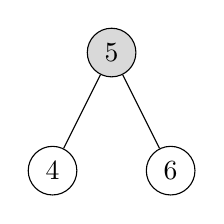
\begin{tikzpicture}
      \node[circle,draw,fill=gray!30](z){5}
      child{ node[circle,draw]{4} }
      child{
        node[circle,draw]{6} child[missing] child[missing] };
    \end{tikzpicture}
    \caption{}
    \label{fig:insert_1}
  \end{subfigure}%
  \begin{subfigure}{.3\textwidth}
    \centering
    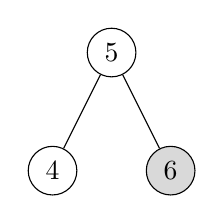
\begin{tikzpicture}
      \node[circle,draw](z){5}
      child{ node[circle, draw]{4} }
      child{
        node[circle,draw,fill=gray!30]{6} child[missing] child[missing] };
    \end{tikzpicture}
    \caption{}
    \label{fig:insert_2}
  \end{subfigure}%
  \begin{subfigure}{.3\textwidth}
    \centering
    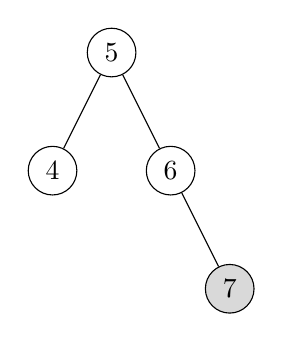
\begin{tikzpicture}
      \node[circle,draw](z){5}
      child{ node[circle, draw]{4} }
      child{
        node[circle,draw]{6} child[missing] child{node[circle,draw,fill=gray!30]{7}} };
    \end{tikzpicture}
    \caption{}
    \label{fig:insert_3}
  \end{subfigure}
  \caption{Insertion operation in a binary search tree.}
  \label{fig:insert_demo}
\end{figure}

Search, insertion and retrieval can be done recursively. Starting at the root node, the input key and the node key are compared: if the input key is smaller,
the operation is done recursively on the left subtree; if the input key is larger, then the operation is done recursively on the right subtree. Figure \ref{fig:insert_demo} shows 
a node with key 7 being inserted into a binary search tree. At \ref{fig:insert_demo}(\ref{sub@fig:insert_1}), the new node is compared to the root. As $7 > 5$, the operation continues at 
the right subtree. At \ref{fig:insert_demo}(\ref{sub@fig:insert_2}) the comparison is done again. As $7 > 6$, the operation continues at the right subtree. Because the node 6 doesn't have any children and $7 > 6$,
a new right child node is created.

\subsection{Balance and rotation}
An AVL tree is based on a binary search tree, with one very important distinction - it is \textit{balanced}. To define what it means for a tree to be balanced, I will first
define what the \textit{height} of a tree is.

\begin{definition}[Tree height]
  \label{def:height}
  The height of a tree is the length of the longest path from the root to a leaf.
\end{definition} 
 
Balance is reliant on this definition - an AVL tree is only balanced when the 
heights of any given left and right child subtrees does not differ by more than one \cite{avl:original}. By keeping balance, the structure ensures that there is a high ratio between the number of 
nodes in the tree and the height. This allows for retrieval and search operations to be done in $O(\log n)$ time in the worst case, with $n$ being the amount of nodes in a tree \cite{avl:computer}.

During the insertion operation, the tree can become imbalanced, which can be mitigated
with either a right rotation or a left rotation. 

\section{Deletion}
\input{content/avl/deletion.tex}